\section{Testing \& Usage}

\subsection{Usage}

The current produced binary accepts the following flags
\texttt{-d}, \texttt{-l}, \texttt{-p}. \texttt{-d} is currently
disabled, \texttt{-l} prints each of the lexemes generated by
the source and \texttt{-p} outputs the AST both before and after
preprocessing.

\subsection{The Lexer, Parser \& Semantic Analyser}

As discussed in previous sections all the phases which are
capable of producing errors or warnings are either doing so
manually using \texttt{fmt::println(stderr, ...)} or using some
customised methods like \texttt{error(...)} or
\texttt{warning(...)}. Additionally, as described in previous
sections as well, the lexer, parser and analyser should not fail
upon the first inconsistency within the program, instead they
should proceed to a state in which they continue processing
normally.

The main aim of testing will be to make sure that both correct
and incorrect input produce the expected behaviour.

\subsubsection{Lexical Analysis}

\begin{figure}[H]
\centering
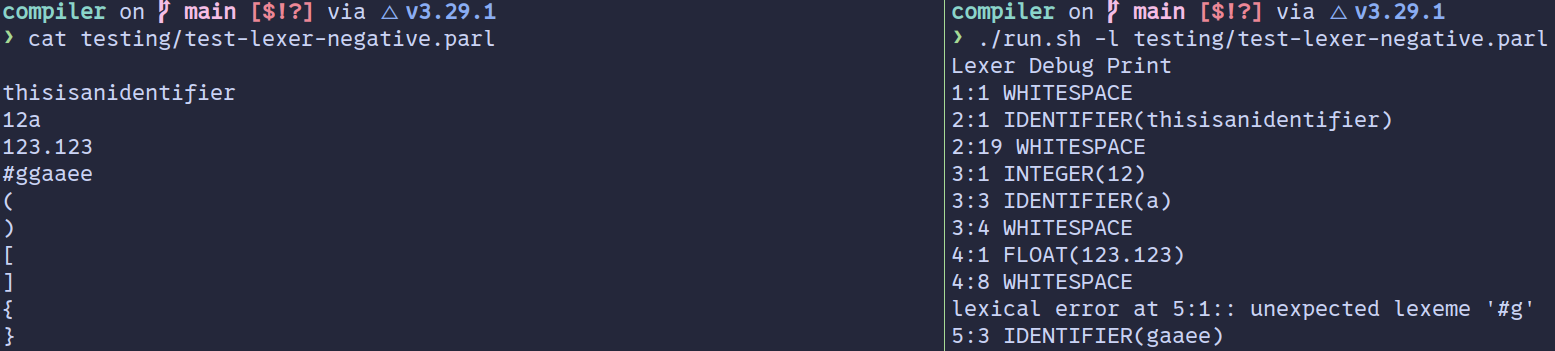
\includegraphics[width=\linewidth]{lexernegative.png}
\caption{Running the negative lexer test
(testing/test-lexer-negative.parl)}
\end{figure}

For lexical analysis two major tests where used,
testing/test-lexer-negative.parl and
testing/test-lexer-positive.parl. Additional, tests include,
testing/test1.parl upto testing/test9.parl.

\subsubsection{Parsing}

\begin{figure}[H]
\centering
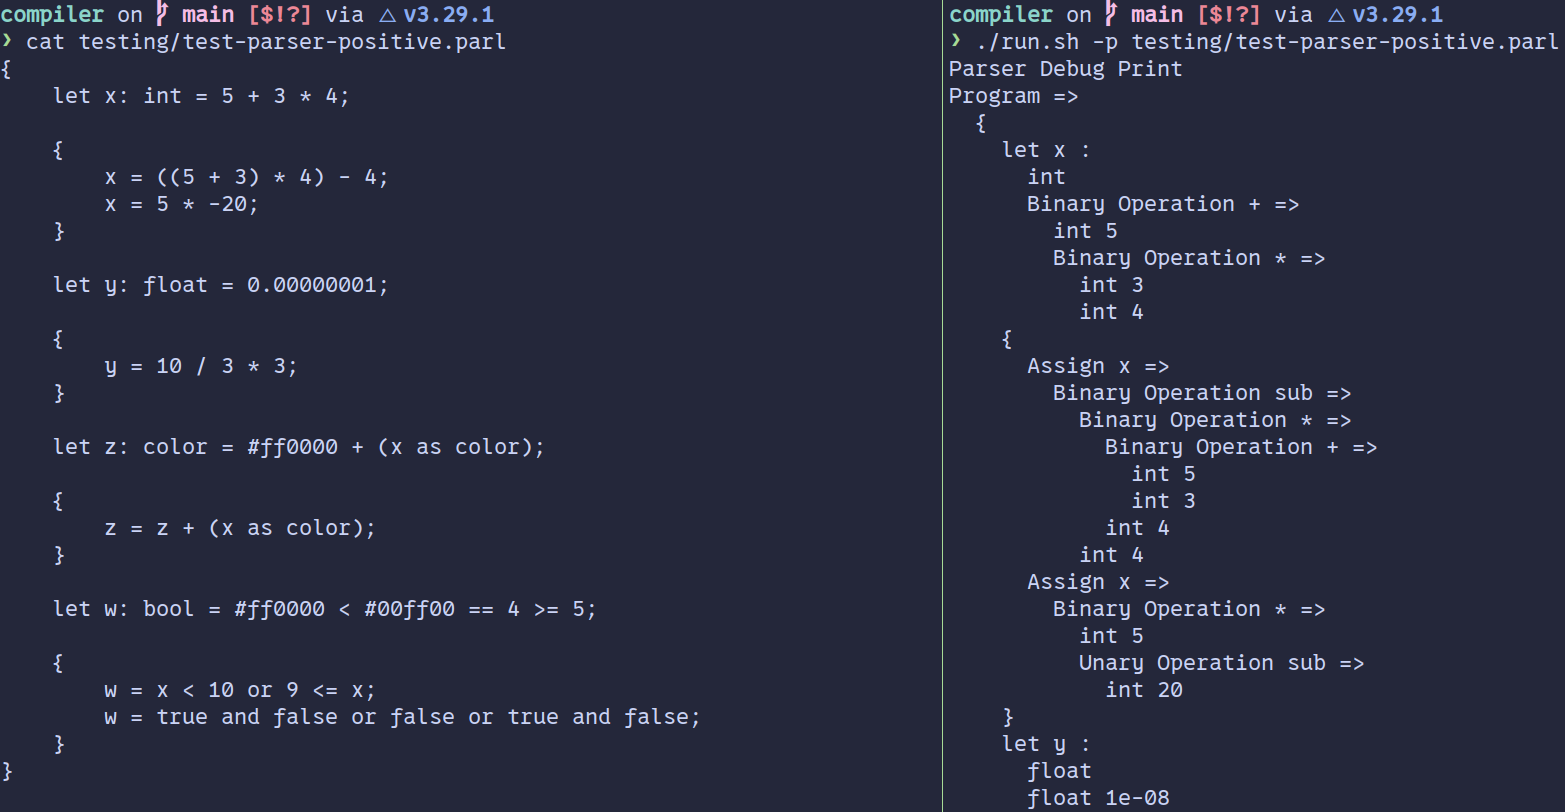
\includegraphics[width=\linewidth]{parserpositive.png}
\caption{Running the positive parser test
(testing/test-parser-positive.parl)}
\end{figure}

Again for parsing two major tests where developed
testing/test-parser-negative.parl and
testing/test-parser-positive.parl.

\begin{figure}[H]
\centering
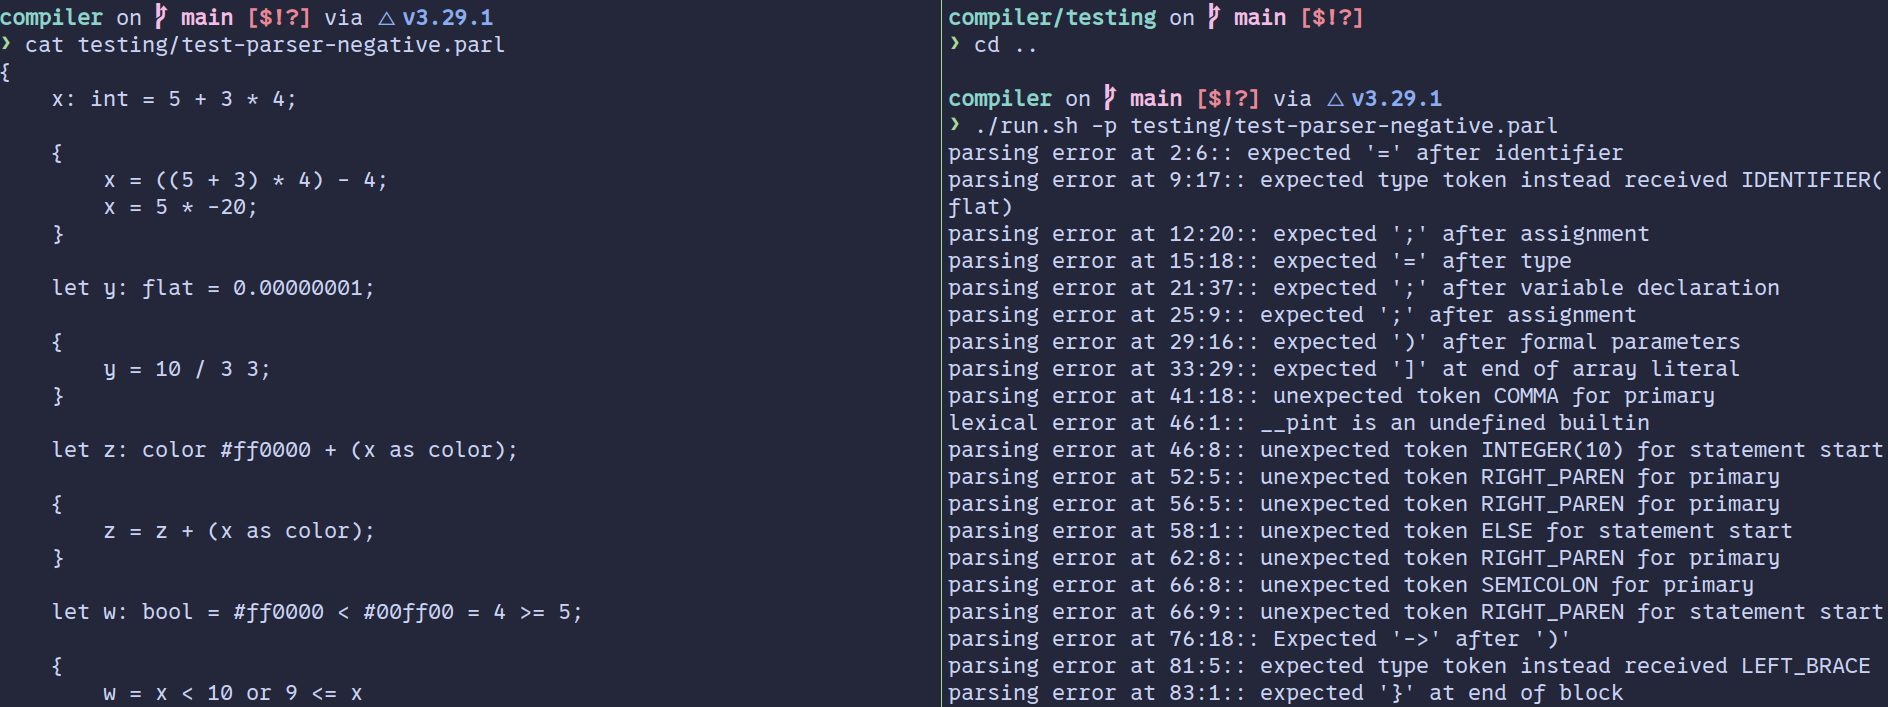
\includegraphics[width=\linewidth]{parsernegative.png}
\caption{Running the negative parser test
(testing/test-parser-negative.parl)}
\end{figure}

In particular the positive test covers of the happy paths of the
parser. However, there are way more possibilities where the
parser flags the input as not conforming to the grammar. Hence,
not all possible code paths are being tested with the negative
test. Additional, files used for testing during development
include: testing/test10.parl, testing/test15.parl and
testing/test16.parl.

\subsubsection{Semantic Analysis}

Semantic analysis is again a leap in complexity and leap in the
order of possible errors and issues. Hence, completely testing
all possible scenarios is very diffcult. Instead the tested
presented and mentioned are those tested written during
development to test certain aspects of the semantic analyser as
it was being developed.

The tests mentioned above are:

\begin{itemize}
    \item testing/test13.parl;
    \item testing/test14.parl;
    \item testing/test17.parl;
    \item testing/test18.parl (parameter types);
    \item testing/test19.parl (parameter types);
    \item testing/test21.parl (casting);
    \item testing/test23.parl (no main functions);
    \item testing/test24.parl (for nested functions);
    \item testing/test25.parl;
    \item testing/test28.parl (for unreachable code);
    \item testing/test31.parl (for arrays);
    \item testing/test32.parl;
    \item testing/test33.parl;
    \item testing/test41.parl (for unreachable code).
\end{itemize}
